\documentclass[a4paper]{article}
\usepackage[a4paper, margin=1in]{geometry} % Adjust margin here, e.g., 1 inch
% Some basic packages
\usepackage[utf8]{inputenc}
\usepackage[T1]{fontenc}
\usepackage{textcomp}
\usepackage[english]{babel}
\usepackage{url}
\usepackage{graphicx}
\usepackage{float}
\usepackage{booktabs}
% \usepackage{enumitem}
\usepackage{enumerate}
\usepackage[colorlinks]{hyperref}

\pdfminorversion=7

% Don't indent paragraphs, leave some space between them
\usepackage{parskip}
\usepackage{changepage}

% Hide page number when page is empty
\usepackage{emptypage}
\usepackage{subcaption}
\usepackage{multicol}
\usepackage[dvipsnames]{xcolor}

% Other font I sometimes use.
% \usepackage{cmbright}

% Math stuff
\usepackage{amsmath, amsfonts, mathtools, amsthm, amssymb}

% Add this line to make equation numbering follow section
\numberwithin{equation}{section}

% Fancy script capitals
\usepackage{mathrsfs}
\usepackage{cancel}
% Bold math
\usepackage{bm}
% Some shortcuts
\newcommand\N{\ensuremath{\mathbb{N}}}
\newcommand\R{\ensuremath{\mathbb{R}}}
\newcommand\Z{\ensuremath{\mathbb{Z}}}
\renewcommand\O{\ensuremath{\emptyset}}
\newcommand\Q{\ensuremath{\mathbb{Q}}}
\newcommand\C{\ensuremath{\mathbb{C}}}

% Easily typeset systems of equations (French package)
\usepackage{systeme}

% Put x \to \infty below \lim
\let\svlim\lim\def\lim{\svlim\limits}

%Make implies and impliedby shorter
\let\implies\Rightarrow
\let\impliedby\Leftarrow
\let\iff\Leftrightarrow
% \let\epsilon\varepsilon

% COURSE SPECIFICS
% GRIFFITHS
\ifdefined\pdfliteral
    \let\griffPdfliteral\pdfliteral
\else \def\griffPdfliteral#1{\special{pdf: literal #1}} \fi

\newcommand\griffr[1][2]{\leavevmode\hbox{\kern1pt\vbox to1ex{}\griffPdfliteral{%
    q 1 J .27 0 0 .27 0 0 cm #1 w
    0 2 m
    0 2 8.1 9.7 9.2 13.2 c
    10.4 16.8 8.4 15.4 8 14.7 c
    7.6 14 6.8 12.6 12 13 c
    17 13.5 14.5 7.8 13.7 6 c
    12.8 4.3 10.3 1.2 11.4 .2 c
    12.6 -.7 18.8 3.6 18.8 3.6 c
    18.8 3.6 l S Q
}\kern6pt}}
\newcommand\hatgriffr{\skew3\hat{\griffr[4]}}

% Add \contra symbol to denote contradiction
\usepackage{stmaryrd} % for \lightning
\newcommand\contra{\scalebox{1.5}{$\lightning$}}

% \let\phi\varphi

% Command for short corrections
% Usage: 1+1=\correct{3}{2}

\definecolor{correct}{HTML}{009900}
\newcommand\correct[2]{\ensuremath{\:}{\color{red}{#1}}\ensuremath{\to }{\color{correct}{#2}}\ensuremath{\:}}
\newcommand\green[1]{{\color{correct}{#1}}}

% horizontal rule
\newcommand\hr{
    \noindent\rule[0.5ex]{\linewidth}{0.5pt}
}

% hide parts
\newcommand\hide[1]{}

% si unitx
\usepackage{siunitx}
\sisetup{locale = FR}

% Environments
\makeatother
% For box around Definition, Theorem, ...
% \usepackage{mdframed}
\usepackage[framemethod=TikZ]{mdframed}

% Custom command to draw a rectangular border around an equation
\setlength{\fboxsep}{5pt}  % Adjust padding inside the box
\usepackage{empheq}
\newcommand*\widefbox[1]{\fbox{\hspace{1em}#1\hspace{1em}}}

\usepackage{environ}  % This package allows for easier custom environment definitions

% Define the custom environment
\NewEnviron{framed}{%
  \begin{empheq}[box=\fbox]{align}
  \BODY
  \end{empheq}
}
% Custom environment to box align equations
% \newenvironment{boxedalign}
%   {\begin{empheq}[box=\fbox]{align}}
%   {\end{align}\end{empheq}}

\newtheorem{thm}{Theorem}[subsection]
\newtheorem{defi}[thm]{Definition}
\newtheorem{lem}[thm]{Lemma}
\newtheorem{ret}{Correction}


\newtheorem*{term}{Terminology}
\newtheorem*{key}{Keywords and Related Concepts}
\newtheorem{lign}[thm]{Equation}
\newtheorem{law}[thm]{Law / Principle}

\usepackage{mathtools}
\DeclarePairedDelimiter\bra{\langle}{\rvert}
\DeclarePairedDelimiter\ket{\lvert}{\rangle}
\DeclarePairedDelimiterX\braket[2]{\langle}{\rangle}{#1\,\delimsize\vert\,\mathopen{}#2}


% \newcounter{theo}[section]
% \renewcommand{\thetheo}{\arabic{section}.\arabic{theo}}

% \mdfsetup{skipabove=1em,skipbelow=0em}
% \theoremstyle{definition}
% \newmdtheoremenv[nobreak=true]{definition}{Definition}
% \newmdtheoremenv[nobreak=true]{theorem}{Theorem}
% \newmdtheoremenv[nobreak=true]{corollary}{Corollary}
% \newmdtheoremenv[nobreak=true]{lemma}{Lemma}

% \newtheorem*{observation}{Observation}
% \newtheorem*{property}{Property}
% \newtheorem*{postulate}{Postulate}
% \newtheorem*{conclusion}{Conlusion}
% \newtheorem*{repitition}{Repitition}
% \newtheorem*{example}{Example}
% \newtheorem*{question}{Question}
% \newtheorem*{intuition}{Intuition}

% End example and intermezzo environments with a small diamond (just like proof
% environments end with a small square)
% \usepackage{etoolbox}
% \AtEndEnvironment{example}{\null\hfill$\diamond$}%
% \AtEndEnvironment{repitition}{\null\hfill$\diamond$}%
% \AtEndEnvironment{opmerking}{\null\hfill$\diamond$}%

% Fix some spacing
% http://tex.stackexchange.com/questions/22119/how-can-i-change-the-spacing-before-theorems-with-amsthm
\makeatletter
\def\thm@space@setup{%
  \thm@preskip=\parskip \thm@postskip=0pt
}


% Exercise 
% Usage:
% \oefening{5}
% \suboefening{1}
% \suboefening{2}
% \suboefening{3}
% gives
% Oefening 5
%   Oefening 5.1
%   Oefening 5.2
%   Oefening 5.3
\newcommand{\exercise}[1]{%
    \def\@exercise{#1}%
    \subsection*{Exercise #1}
}

\newcommand{\subexercise}[1]{%
    \subsubsection*{Exercise \@exercise.#1}
}

\usepackage{xcolor}
\newcommand{\textred}[1]{\textcolor{red}{#1}}

% \lecture starts a new lecture (les in dutch)
%
% Usage:
% \lecture{1}{di 12 feb 2019 16:00}{Inleiding}
%
% This adds a section heading with the number / title of the lecture and a
% margin paragraph with the date.

% I use \dateparts here to hide the year (2019). This way, I can easily parse
% the date of each lecture unambiguously while still having a human-friendly
% short format printed to the pdf.

\usepackage{xifthen}
\def\testdateparts#1{\dateparts#1\relax}
\def\dateparts#1 #2 #3 #4 #5\relax{
    \marginpar{\small\textsf{\mbox{#1 #2 #3 #5}}}
}

\def\@lecture{}%
\newcommand{\lecture}[3]{
    \ifthenelse{\isempty{#3}}{%
        \def\@lecture{Lecture #1}%
    }{%
        \def\@lecture{Lecture #1: #3}%
    }%
    \subsection*{\@lecture}
    \marginpar{\small\textsf{\mbox{#2}}}
}

\def\@chapter{}%
\newcommand{\chapter}[3]{
    \ifthenelse{\isempty{#3}}{%
        \def\@chapter{Chapter #1}%
    }{%
        \def\@chapter{Chapter #1: #3}%
    }%
    \subsection*{\@chapter}
    \marginpar{\small\textsf{\mbox{#2}}}
}

\def\@week{}%
\newcommand{\week}[3]{
    \ifthenelse{\isempty{#3}}{%
        \def\@week{Uge #1}%
    }{%
        \def\@week{Uge #1: #3}%
    }%
    \subsection*{\@week}
    \marginpar{\small\textsf{\mbox{#2}}}
}

% These are the fancy headers
% \usepackage{fancyhdr}
% \pagestyle{fancy}

% LE: left even
% RO: right odd
% CE, CO: center even, center odd
% My name for when I print my lecture notes to use for an open book exam.
% \fancyhead[LE,RO]{Gilles Castel}

% \setlength{\headheight}{5pt}

% % \fancyhead[R]{\@lecture} % Right odd,  Left even
% \fancyfoot[R]{\thepage}  % Right odd,  Left even
% \fancyfoot[C]{\leftmark}     % Center

\makeatother

% Todonotes and inline notes in fancy boxes
\usepackage{todonotes}
\usepackage{tcolorbox}

% Make boxes breakable
\tcbuselibrary{breakable}

% Usage: 
% \begin{correction}
%     Lorem ipsum dolor sit amet, consetetur sadipscing elitr, sed diam nonumy eirmod
%     tempor invidunt ut labore et dolore magna aliquyam erat, sed diam voluptua. At
%     vero eos et accusam et justo duo dolores et ea rebum. Stet clita kasd gubergren,
%     no sea takimata sanctus est Lorem ipsum dolor sit amet.
% \end{correction}
\newenvironment{correction}{\begin{tcolorbox}[
    arc=0mm,
    colback=white,
    colframe=green!60!black,
    title=Correction,
    fonttitle=\sffamily,
    breakable
]}{\end{tcolorbox}}

% Same as 'correction' but color of box is different
\newenvironment{note}{\begin{tcolorbox}[
    arc=0mm,
    colback=white,
    colframe=white!60!black,
    title=Note,
    fonttitle=\sffamily,
    breakable
]}{\end{tcolorbox}}


% Figure support as explained in my blog post.
\usepackage{import}
\usepackage{xifthen}
\usepackage{pdfpages}
\usepackage{transparent}
\newcommand{\incfig}[1]{%
    \def\svgwidth{\columnwidth}
    \import{./figures/}{#1.pdf_tex}
}

% Fix some stuff
% %http://tex.stackexchange.com/questions/76273/multiple-pdfs-with-page-group-included-in-a-single-page-warning
\pdfsuppresswarningpagegroup=1


% My name
\author{Erik Bach Ryhl}


\graphicspath{ {./figs/} {./figs/talks/what-is-a-topological-insulator}}

\setcounter{tocdepth}{4}
\setcounter{secnumdepth}{3}

\usepackage{caption}
\usepackage{subcaption}

\title{Topological Insulators}
\begin{document}
    \maketitle
    \tableofcontents
    \newpage

    \section{An unprecise introduction}
    \subsection{What is an insulator?}
    On the most general level, an insulator is something that does not transmit current. In other words, it can be seen as the opposite of a conductor.
    
    But it is of course not as simple as that, because we can have things that are insulating sometimes and conducting at other times. Very superficially, a semiconductor is an example of something that is conducting at finite temperatures while insulating at zero temperature.

    The unwillingnes of an insulator to conduct electricity, which really means that it doesn't like electrons moving about, is a quantum mechanical effect. 

    \subsection{Band Structure and the Fermi Level: How Topology Enters the Picture}
    Quantum mechanically, an atom has multiple spin orbitals and even different kinds (\(s, p, d\) and \(f\) orbitals). Since electrons are leptons, which means that they are spin-\(1/2\) fermions, they obey the \href{https://en.wikipedia.org/wiki/Pauli_exclusion_principle}{Pauli exclusion principle}, which says that two fermions cannot share the same four quantum numbers simultaneously. If two electrons are in the same orbital, this would mean that they share three out of four quantum numbers. The only one left is the spin, and thus two electrons cannot have the same spin if they occupy the same orbital. And since the only two possible spins for an electron is \(\pm 1 / 2\), we conclude that each orbital can host one spin-up electron and one spin-down electron simultaneously.

    This is the case for a single atom. But if we put two atoms with only one electron in the relevant orbital (is it just "the outer" that matters, and what does that even mean?) very closely together, the configurations can "hybridize" and make combined states. Some of these will have more delocalized electrons which lower the free energy. I don't know why or how this works, but that's the gist. Take a look at the energy levels at the bottom of figure \ref{fig:electron-bonding-energy}.

    \begin{figure}
        \centering
        \begin{subfigure}[b]{0.45\textwidth}
            \centering
            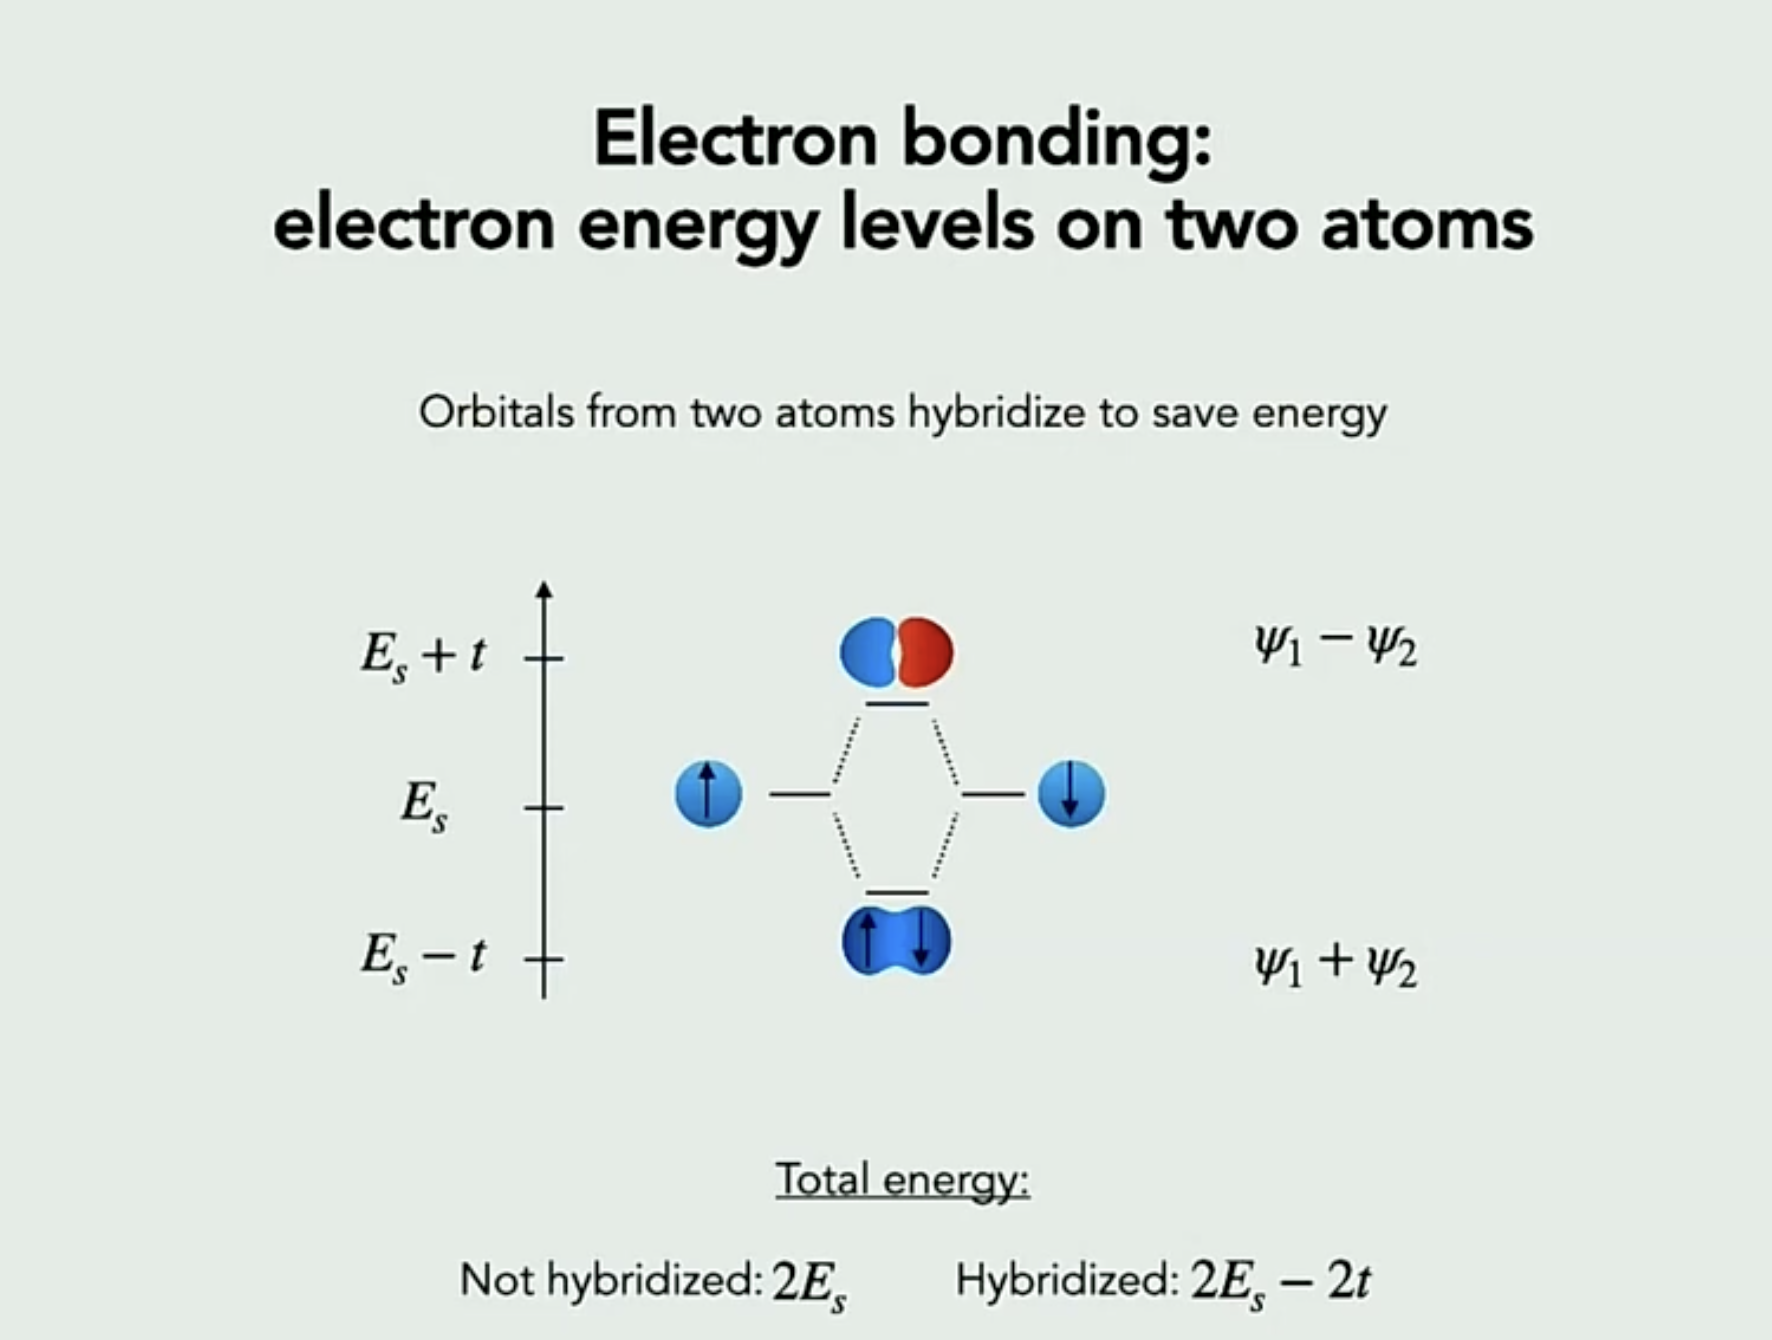
\includegraphics[width=0.9\textwidth]{hybrid-1.png}
            \caption{Two-atom hybridisation}
        \end{subfigure}
        \hfill
        \begin{subfigure}[b]{0.45\textwidth}
            \centering
            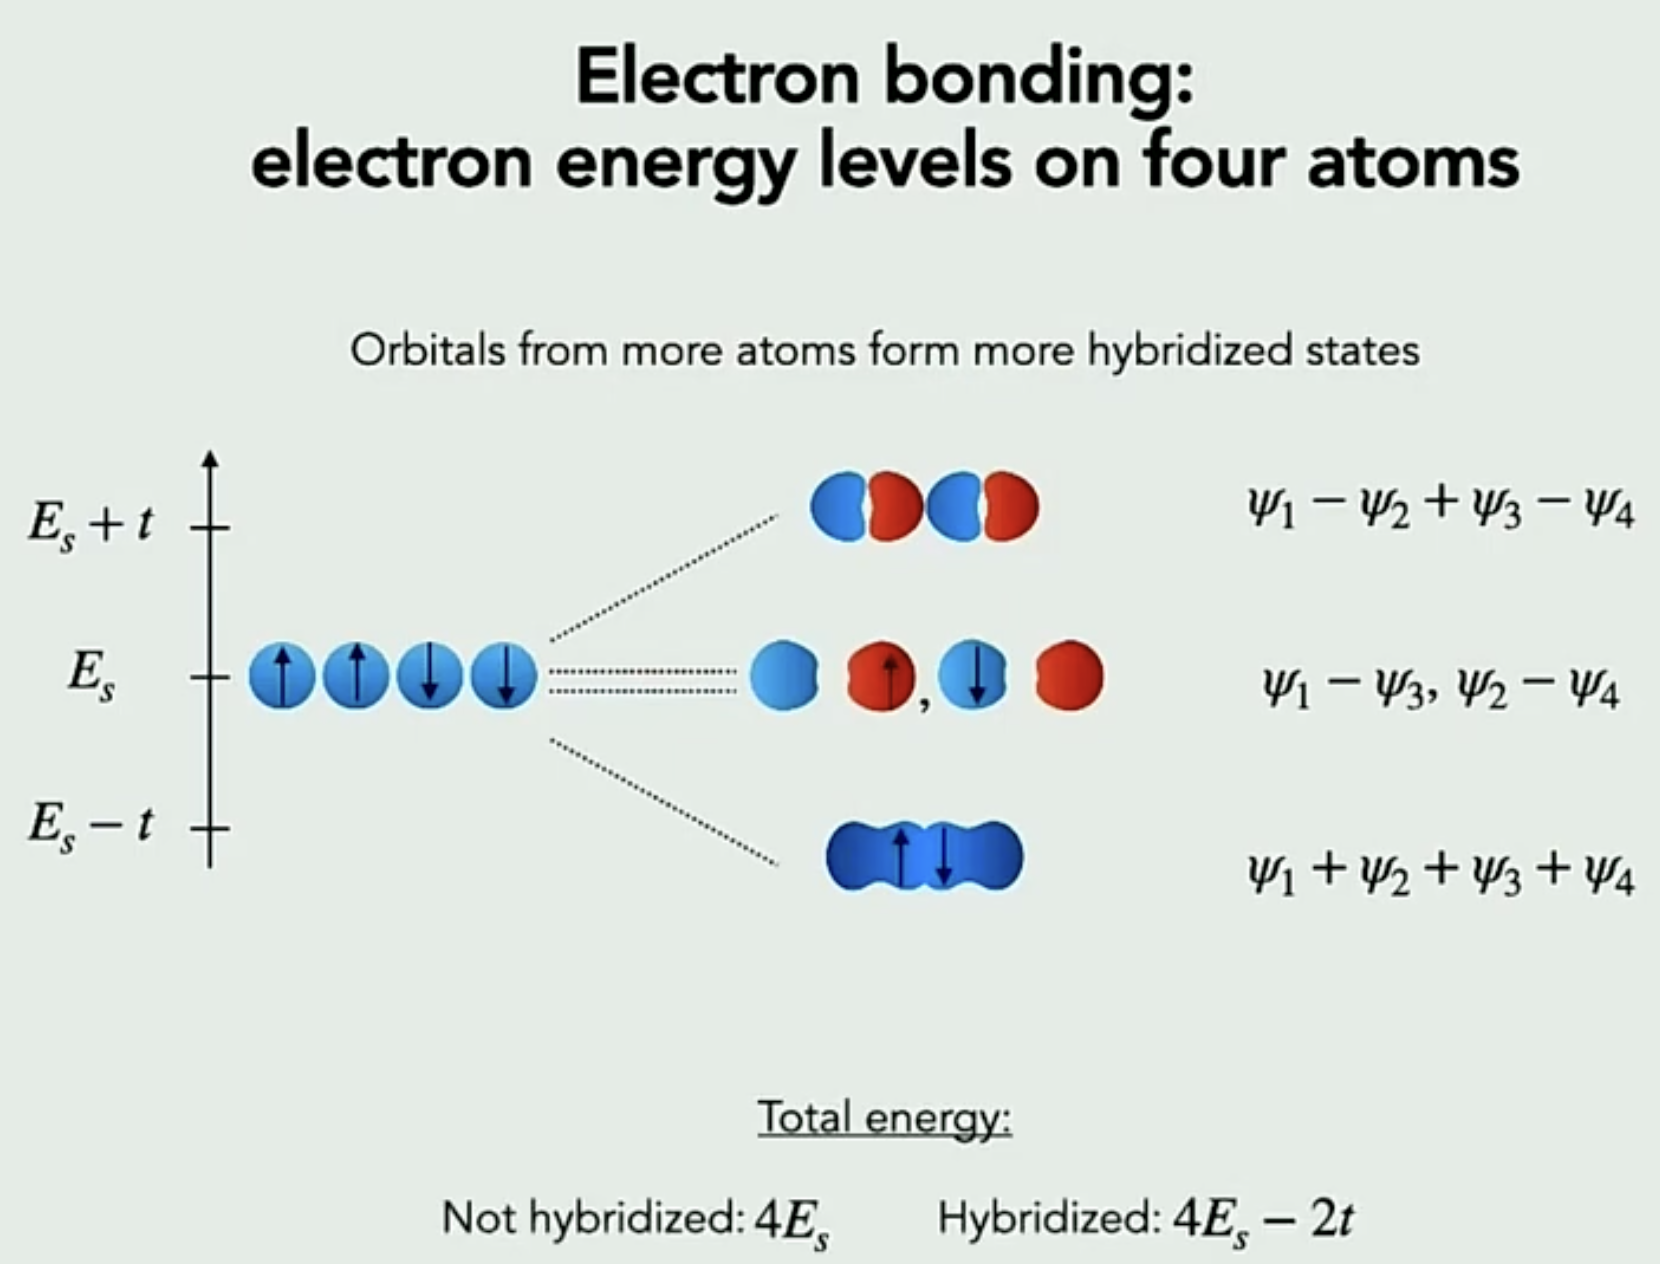
\includegraphics[width=0.9\textwidth]{hybrid-2.png}
            \caption{Four-atom hybridisation}
        \end{subfigure}
        \caption{Energy levels of electron bonding. Credit to talk: \href{https://www.youtube.com/watch?v=YwaF5IC8eBY&ab_channel=KavliInstituteforTheoreticalPhysics}{What is a topological insulator?} - Jennifer Cano}
        \label{fig:electron-bonding-energy}
    \end{figure}

    If we plot the possible energy levels of the system, as the number of closely packed atoms increases, we see the pattern shown in figure \ref{fig:discrete-band-structure}. In the limit, we analytically get a cosine curve (such as with the number of atoms being on the order of \(10^{23} \)). This continuous approximation to the discrete energy levels in the limit is known as the material's \textit{band structure}.

    \begin{figure}[H]
        \centering
        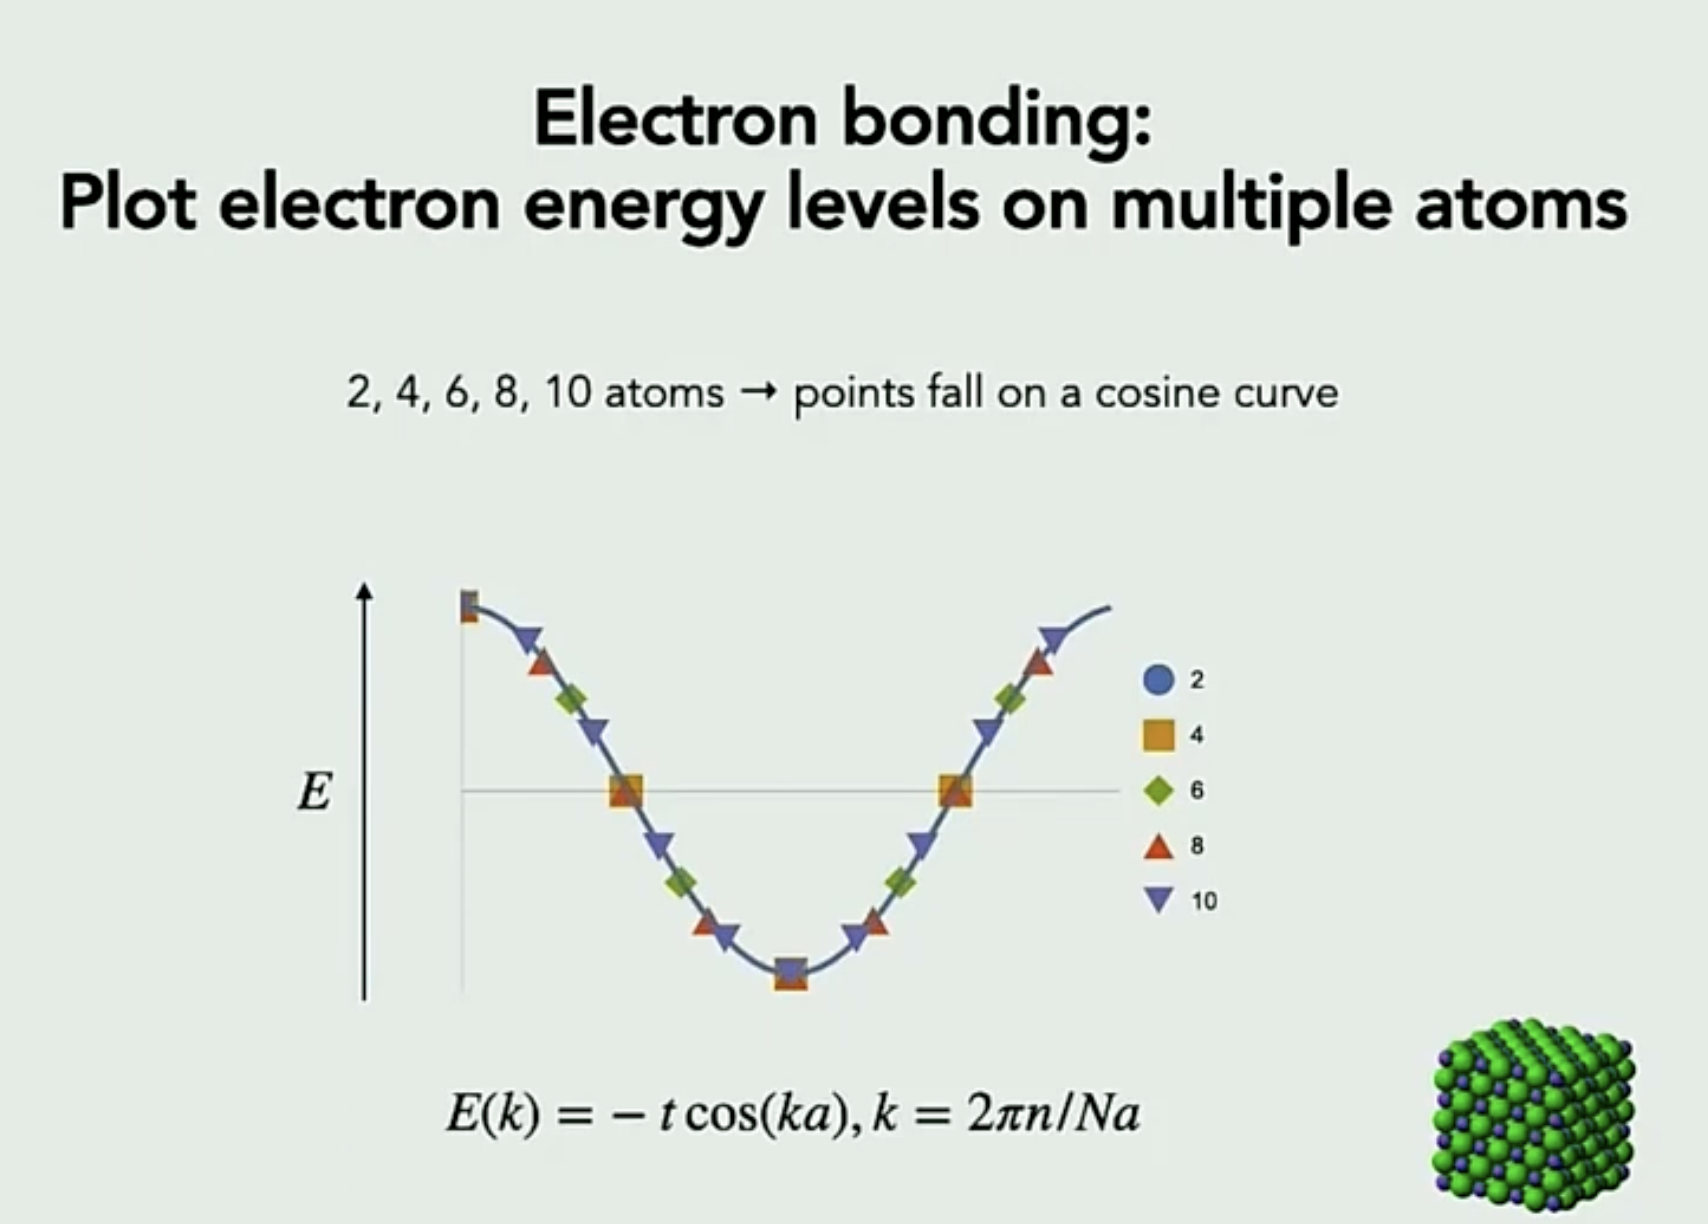
\includegraphics[width=0.8\textwidth]{discrete-band-structure.png}
        \caption{Approximating the discrete band-structure in a crystal we get a continuous line. This is known as the band structure of the material.}
        \label{fig:discrete-band-structure}
    \end{figure}

    For real world materials, we get multiple bands from multiple different orbitals, and the result can be quite complex as seen in figure \ref{fig:band-structure-example}.

    \begin{figure}[H]
        \centering
        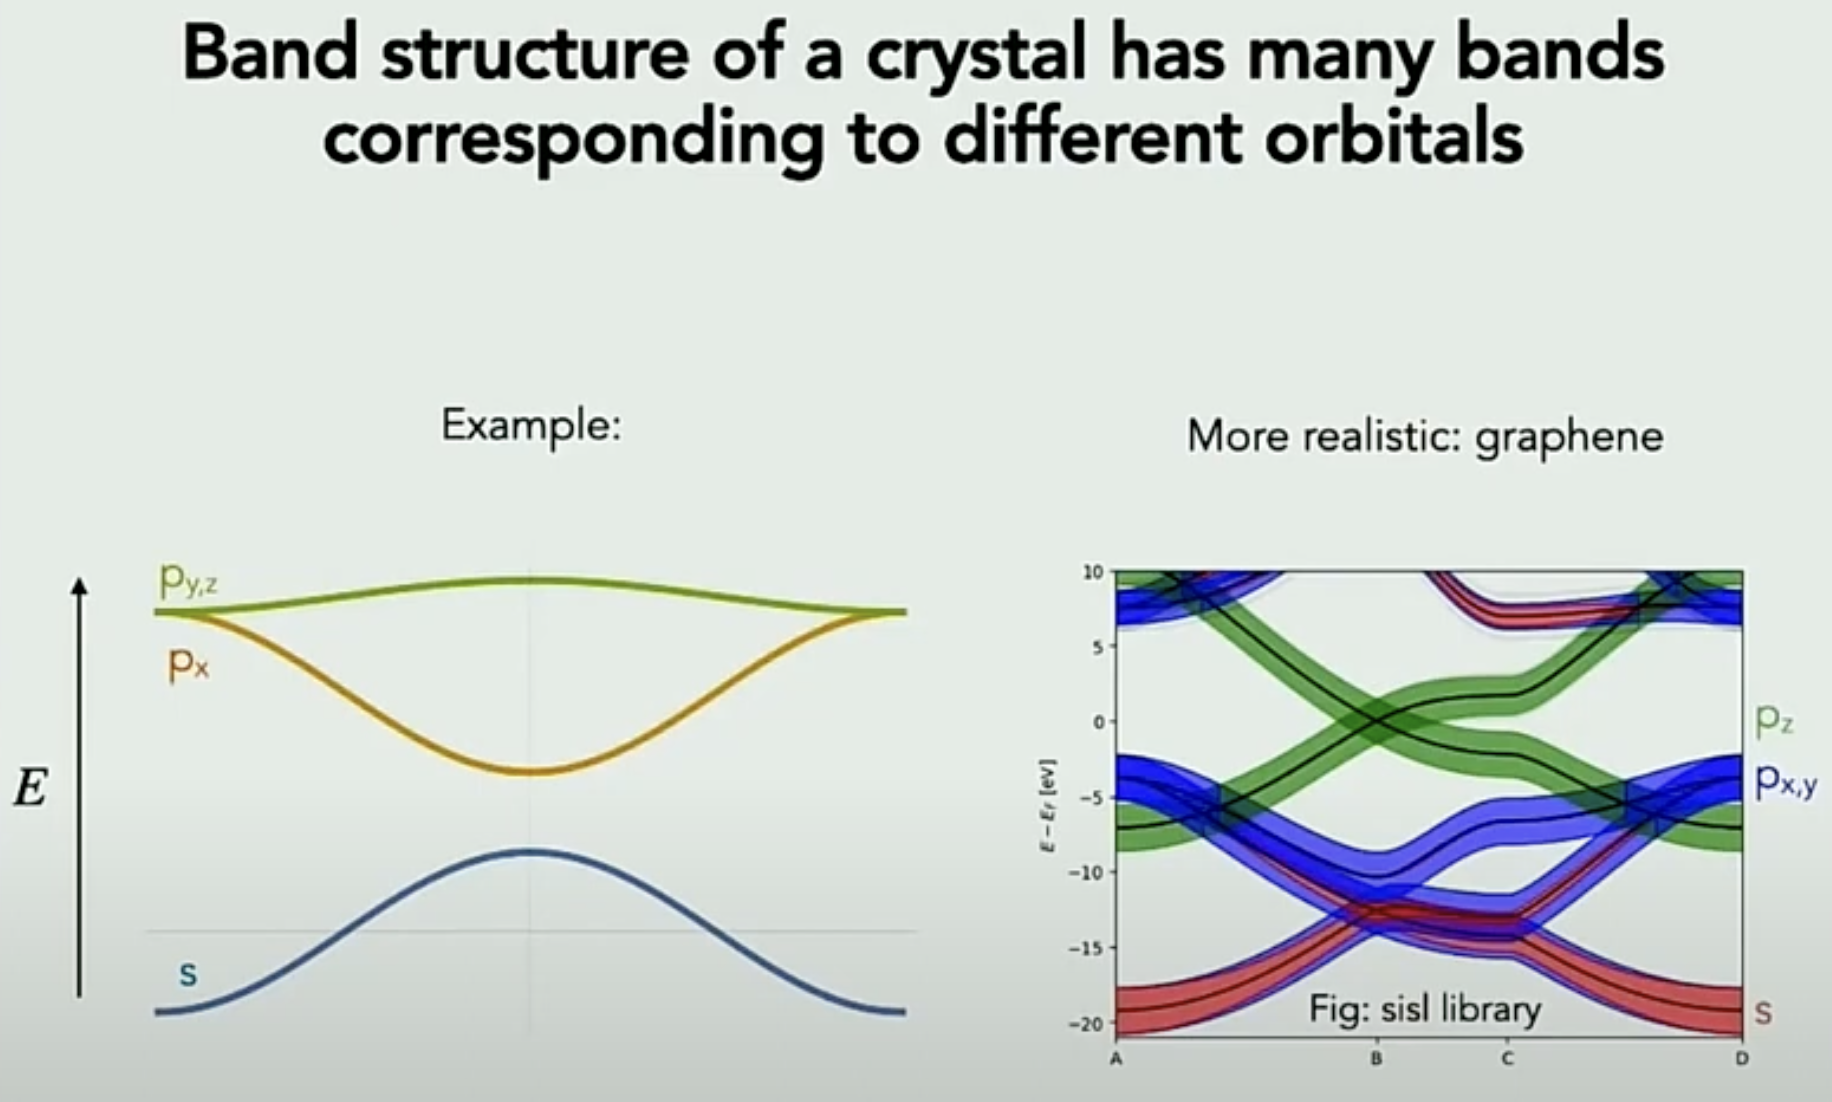
\includegraphics[width=0.8\textwidth]{band-structure-example.png}
        \caption{An abstract example of band structures from multiple orbitals as well as a real-world example from graphene.}
        \label{fig:band-structure-example}
    \end{figure}

    This quantum mechanical view of a material and its band structure allows for a much more precise statement of what an insulator is compared to a conductor (metal). If we draw a horisontal line on the orbital-energy graph, we know that for each energy level, two electrons can in principle occupy it (spin-up and spin-down). 
    
    If we then have an atomic structure where an orbital is only half full, then there will be 

    interpret figure \ref{fig:metal-vs-insulator}

    \begin{figure}[H]
        \centering
        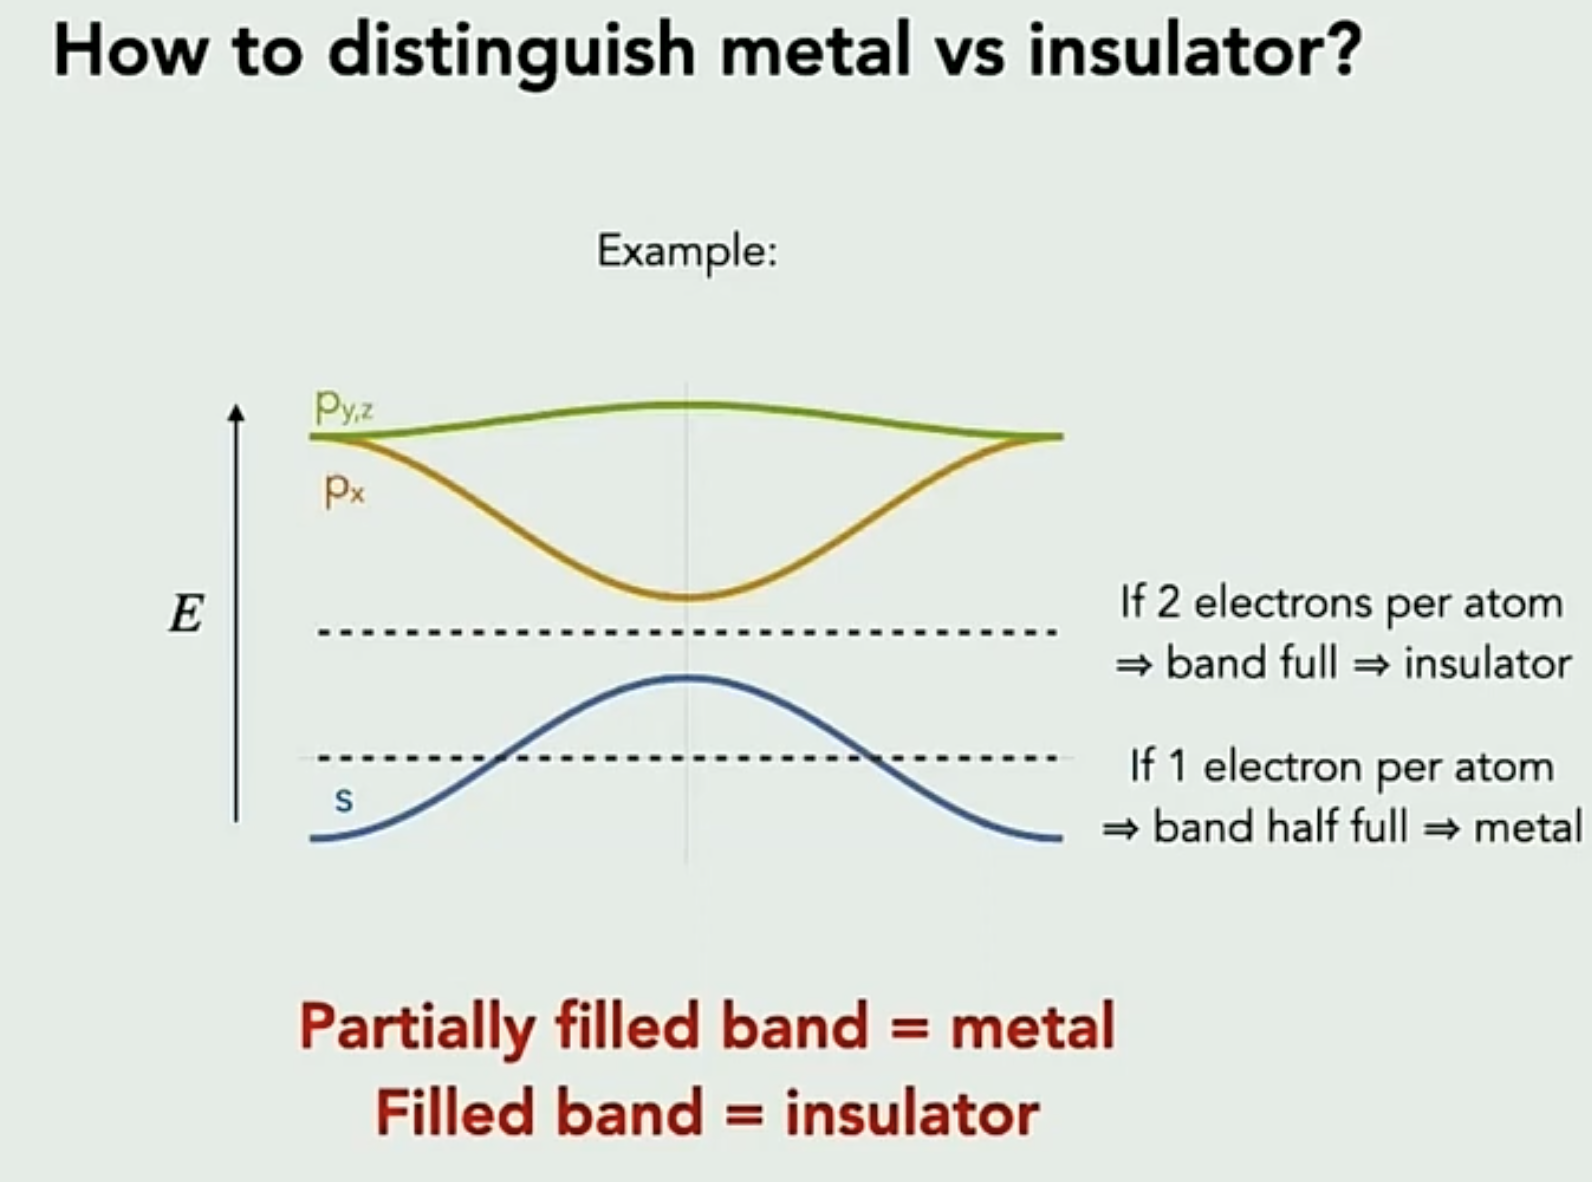
\includegraphics[width=0.8\textwidth]{metal-vs-insulator.png}
        \caption{}
        \label{fig:metal-vs-insulator}
    \end{figure}




    \subsection{Berry Curvature and The Chern Number}
    \subsection{Prediction of the Existence of Gapless Edge States}
    \subsection{Realisations and Possible Interesting Applications}
    \section{Interlude - Basic Quantum Mechanics}
    \subsection{The Schrödinger Equation}
    \subsection{The Hamiltonian of a Quantum Mechanical System}
    \subsection{Pauli Spin Matrices}
    \subsection{Spin-Orbit Coupling and its Hamiltonian}
    \subsection{The Bloch Sphere}
    \subsection{Berry Curvature and The Chern Number Revisited}
    \section{Interlude - Floquet Theory}
    \subsection{Floquet's Theorem}
    \subsection{The Hill Equation and Mathieu's Equation}
    \subsection{Kapitza's Pendulum}
    \subsubsection{Kapitza's Pendulum with Lagrangian Mechanics}
    \subsubsection{Kapitza's Pendulum with Floquet Theory}
    \section{Floquet Engineering - Putting It All Together}
    \subsection{How does Floquet Theory Enter the Picture?}
    \subsection{An Effective Hamiltonian}
    \subsection{Quasienergies}
    \subsection{Floquet-Bloch States}
    \subsection{Current Research and Open Problems}
    \subsubsection{Notes from talk: \href{https://www.youtube.com/watch?v=YwaF5IC8eBY&ab_channel=KavliInstituteforTheoreticalPhysics}{What is a topological insulator?} - Jennifer Cano}
    \begin{figure}[h]
        \centering
        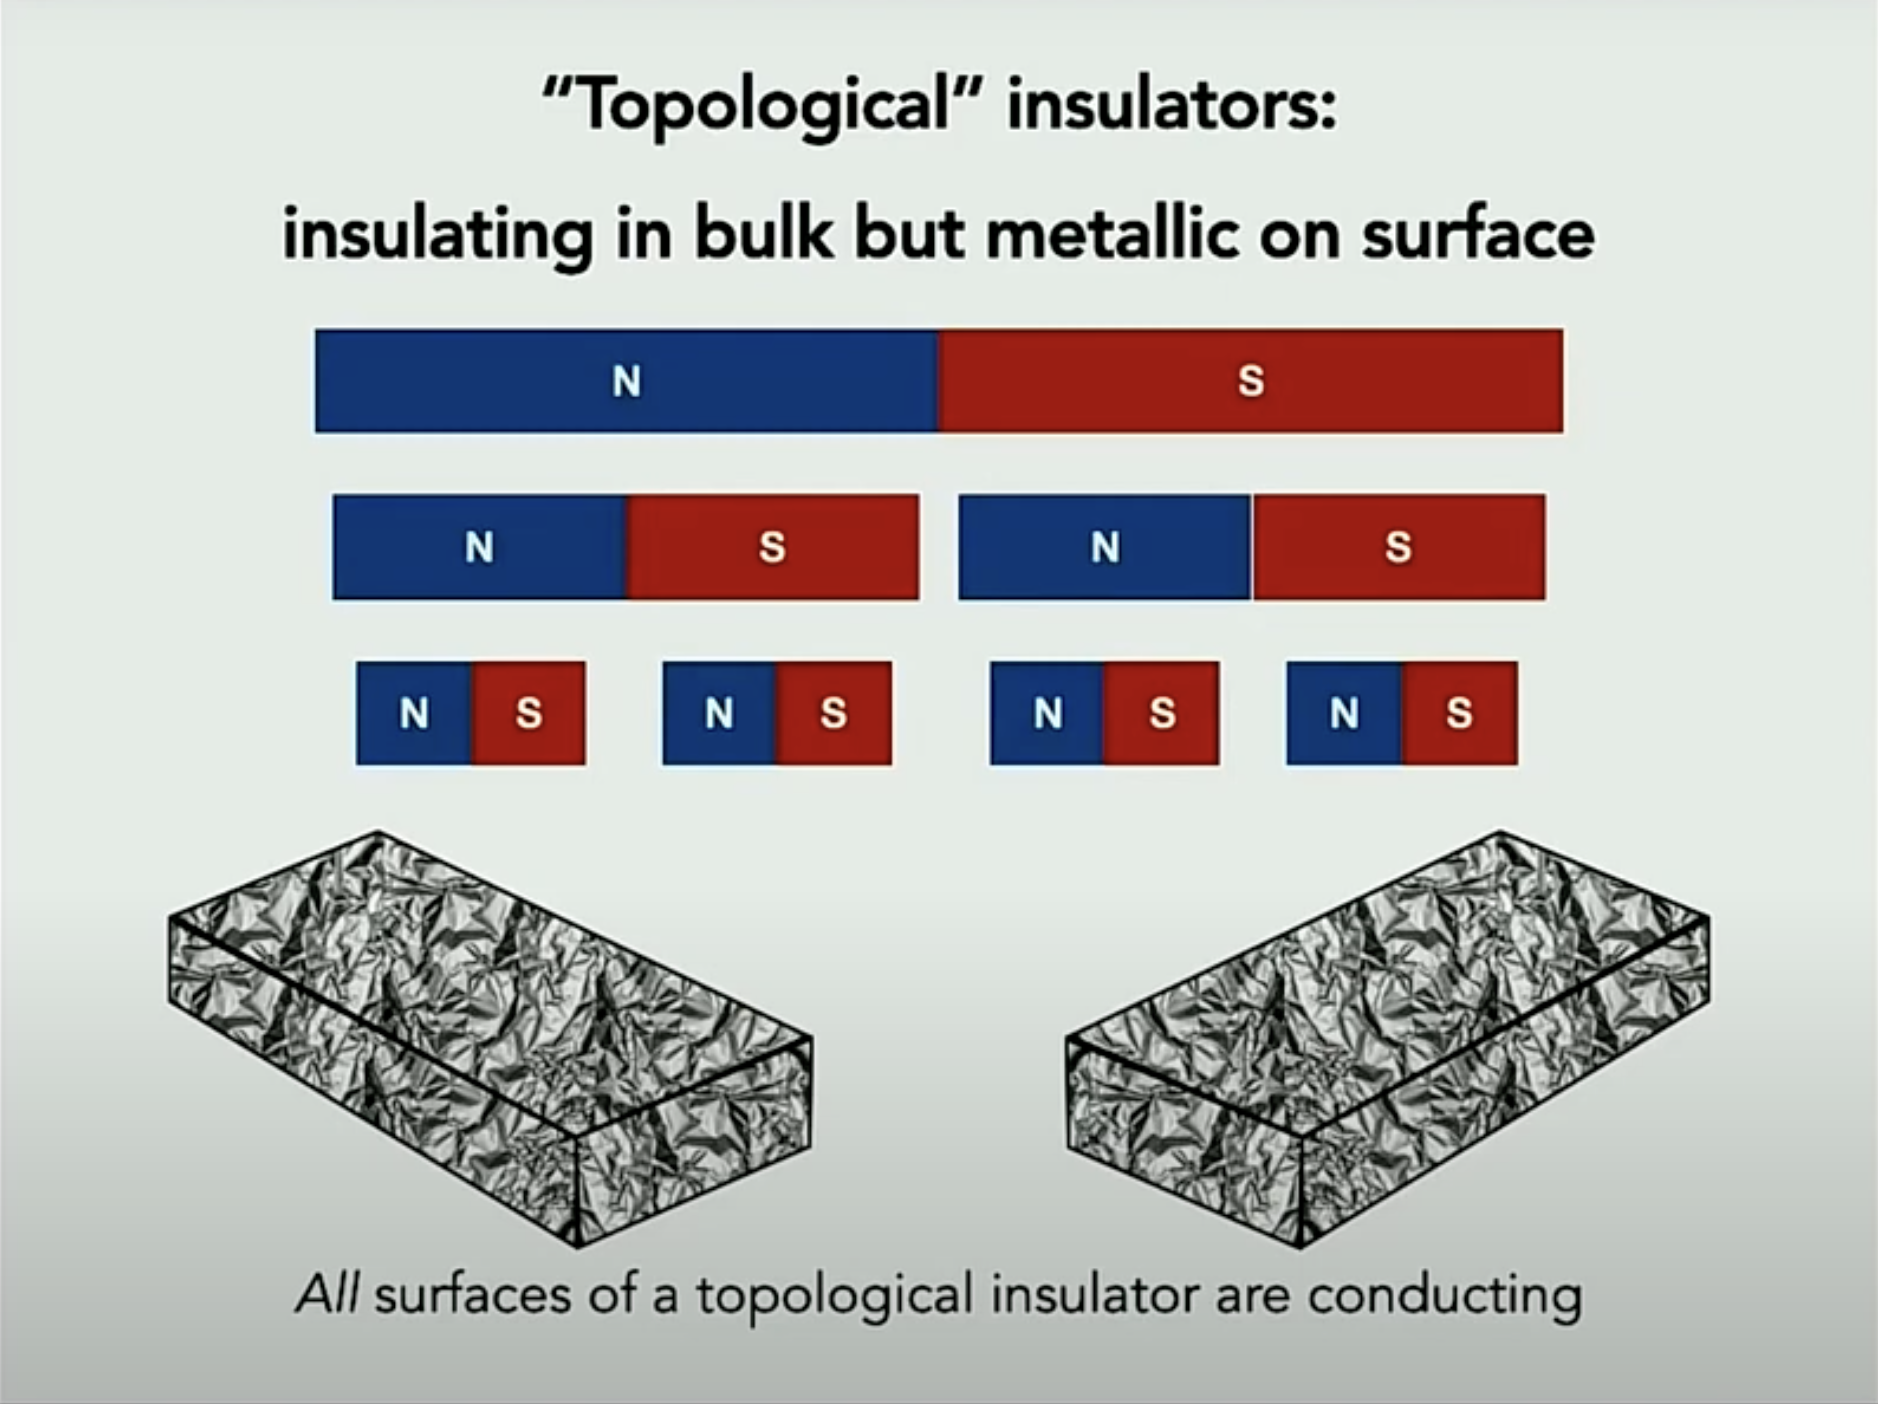
\includegraphics[width=0.8\textwidth]{top-cantor-magnet.png}
        \caption{Image taken from the talk. A topological insulator is conducting on the surface, but insulating in the bulk.}
        \label{fig:top-cantor-magnet}
    \end{figure}
    Thought from Figure \ref{fig:top-cantor-magnet}: When cutting a topological insulator in half, the two new surfaces that was previously in the bulk will become conducting surfaces while the bulk still remains insulating. This is just how you can't split a magnet to get two monopoles. But the diagram of the bar magnets reminds me of a Cantor set - in the limit of splitting the bar magnet, we would get a string of magnetic dipoles spanning the original length. Depending on how we achieve this Cantor set, the spacing will be different. What will the field be from this string of dipoles? Does it depend on the Cantor set spacing? Is it invariant and perfectly "approximated" by the field of the original magnet? And once this has been investigated, how does it compare to the properties that a string of infinitely thin topological insulators would have? Can it be analysed the same way?

    \section{Unstructured topics}
    \subsection{Dirac Cone}
    
    \section{Topological Physics at the Light-Matter Interface}
    \subsection{From the talk}
    Notes for the talk "\href{https://www.youtube.com/watch?v=LjHlAO46i0c&t=0s&ab_channel=AspenPhysics}{Topological Physics at the Light-Matter Interface}" by Professor Gil Refael.

    Keywords mentioned
    \begin{enumerate}
        \item Spin-orbit coupling
        \item Bloch Sphere
        \item Spinor Space
        \item Winding \(g_{\mathbf{p}}\) 
        \item Excitons
        \item Topolariton
        \item Hybridize
        \item Time-reversal symmetry (and breaking)
        \item "Having a periodic drive is like adding an extra dimension to the system" - How should this be understood? How does this relate to Floquet theory and how it is used to make a time-dependent Hamiltonian into an effective time-independent Hamiltonian. Is it like saying that time is usually a dimension which configuration space can be parameterised by and you get a curve with each point along the curve having a point in time (or multiple) associated with it, but then when this curve is periodic, you essentially have a "geometrical shape" traced out again and again, which can then be viewed as the shape in itself without time associated with it - that is, a static picture, where you incoorperate the time axis as an extra dimension where each point in configuration space has infinitely many associated time points, but since it is mod-\(2\pi\) you can associate a "unique" point along the time axis which maps to a unique point on the "geometrical shape". That is, an extra dimension!
        \item BHZ band structure
        \item Pertubative and non-pertubative
    \end{enumerate}

    \subsection{Paper: "Floquet Topological Insulator in Semiconductor Quantum Wells"}
    \begin{enumerate}
        \item Brillouin Zone
        \item 
    \end{enumerate}
    
\end{document}